\documentclass[12pt,a4paper]{article}

% Margins.
\setlength{\oddsidemargin}{0in}
\setlength{\evensidemargin}{0in}
\setlength{\headheight}{12pt}
\setlength{\headsep}{42pt}
\setlength{\topmargin}{-54pt}
\setlength{\textwidth}{6.5in}
\setlength{\textheight}{10in}

\usepackage{amsmath}
\usepackage{float}
\usepackage{graphicx}
\usepackage[hyphens]{url}
\usepackage{hyperref}	% Clickable links to figures, references and urls.
\usepackage{datetime}
\usepackage{longtable}
\usepackage{subfigure}

% Links direct to top of figures.
\usepackage[all]{hypcap}

% Drawing.
\usepackage{pgf}
\usepackage{tikz}

% Listings for formatting code.
\usepackage{listings}
\usepackage{textcomp}
% General options.+++
\lstset{breaklines=true, basicstyle=\small\ttfamily, tabsize=4, numbers=left, stepnumber=1, frame=single, showstringspaces=false, upquote=true}
% C++ specific high-lighting. Comments are 50/50 shades of green/black and strings coloured with 60/40 red/black mixture.
\lstset{language=[ISO]C++, commentstyle=\color{green!50!black}, keywordstyle=\color{blue}, stringstyle=\color{red!60!black}}

%opening
\title{\vspace{-3cm}Physics for Engineers\\Class 41\\Displacement Current: Final Form of Maxwell's Equations}
\author{Attique Dawood}
\date{April 28, 2014\\[0.2cm] Last Modified: \today, \currenttime}
\begin{document}
\maketitle
\section{Announcements}
\begin{itemize}
\item Quiz \#07 today.
\end{itemize}
\section{Faraday's Law}
\begin{equation}
\oint\limits_{L} \textbf{E}\cdot d\textbf{\textit{l}}=-V_{emf}.
\end{equation}
Or
\begin{equation}
\oint\limits_{L} \textbf{E}\cdot d\textbf{\textit{l}}=-\dfrac{d\Phi_B}{dt}.
\end{equation}
For a solenoid with a $N$ number of turns
\begin{equation}
\oint\limits_{L} \textbf{E}\cdot d\textbf{\textit{l}}=-N\dfrac{d\Phi_B}{dt}.
\end{equation}
The standard form better known as the Faraday's Law of Induction is
\begin{equation}
\oint\limits_{L} \textbf{E}\cdot d\textbf{\textit{l}}=-\dfrac{\partial}{\partial t}\int\limits_{S}\textbf{B}\cdot d\textbf{S}.
\end{equation}
\section{Displacement Current}
Consider the two surfaces $S_1$ and $S_2$ shown in figure \ref{displacement-current}. A current flowing in the circuit charges the capacitor. If we consider $S_1$ then applying Ampere's Law we get
\begin{equation}
\oint\limits_{L} \textbf{H}\cdot d\textbf{\textit{l}}=I.
\end{equation}
Which is the conduction current flowing in the wire. But if we consider $S_2$ then no current is cutting $S_2$ so enclosed current comes to be zero. But this is a contradiction since we already know that both are surfaces are bound by the path and we should get same result for $S_1$ or $S_2$.

In order to resolve this contradiction Maxwell introduced an extra term in Ampere's Law known as displacement current. You can think of it as a logical current that must be flowing between capacitor terminals in space. This is different from conduction current we are familiar with. Conduction current is defined as
\begin{equation}
I=\dfrac{d\Phi_D}{dt}=\dfrac{\partial}{\partial t}\int\limits_{S}\textbf{D}\cdot d\textbf{S}.
\end{equation}
Where $\Phi_D$ is defined as electric flux due to \textbf{D}. $\int\limits_{S}\textbf{D}\cdot d\textbf{S}$ is the electric flux and $\textbf{D}=\epsilon\textbf{E}$.
So the final form of Ampere's Law is
\begin{equation}
\oint\limits_{L} \textbf{H}\cdot d\textbf{\textit{l}}=I+\dfrac{\partial}{\partial t}\int\limits_{S}\textbf{D}\cdot d\textbf{S}.
\end{equation}
\begin{figure}[H]
\centering
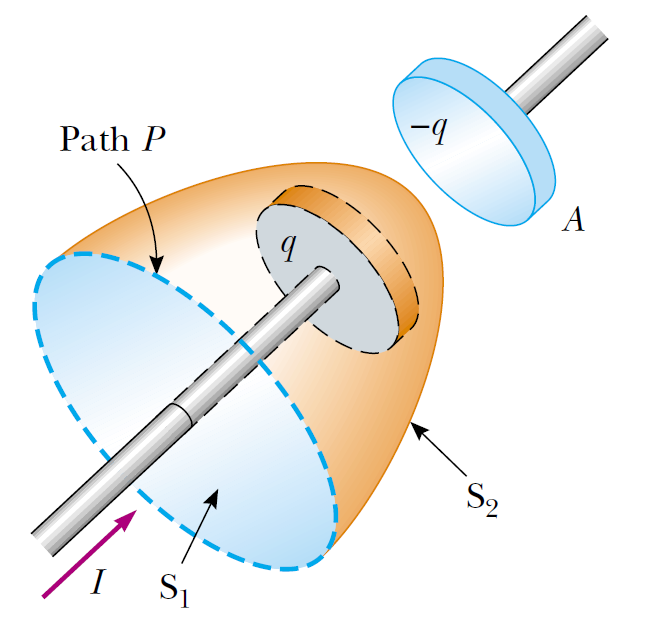
\includegraphics[scale=0.45]{Figure30-25.png}
\caption{Two open surfaces bounded by Amperian path.}
\label{displacement-current}
\end{figure}
\section{Maxwell's Equations in Final Form}
Maxwell's equations in final form are
\subsection{Gauss's Law}
\begin{equation}
\oint\limits_{S} \textbf{D}\cdot d\textbf{S}=q_{enc}.
\end{equation}
\subsection{Faraday's Law}
\begin{equation}
\oint\limits_{L} \textbf{E}\cdot d\textbf{\textit{l}}=-\dfrac{\partial}{\partial t}\int\limits_{S}\textbf{B}\cdot d\textbf{S}.
\end{equation}
\subsection{Ampere's Law}
\begin{equation}
\oint\limits_{L} \textbf{H}\cdot d\textbf{\textit{l}}=I+\dfrac{\partial}{\partial t}\int\limits_{S}\textbf{D}\cdot d\textbf{S}.
\end{equation}
\subsection{Gauss's Law for Magnetism}
\begin{equation}
\oint\limits_{S} \textbf{B}\cdot d\textbf{S}=0.
\end{equation}
The constitutive relations are
\begin{equation}
\textbf{D}=\epsilon\textbf{E}
\end{equation}
and
\begin{equation}
\textbf{B}=\mu\textbf{H}
\end{equation}
\section{Exercises}
\noindent\textbf{Question 1 \cite[Problem 9.4, page 404]{Sadiku}} A magnetic field given by $\textbf{B}=40\cos 10^4 t\hat z$ mW/m$^2$ cuts a current carrying loop. The loop is placed in $xy$--plane and has an area 20 cm$^2$. Find $V_{emf}$ and direction of induced current. What is induced current if current limiting resistor is 4 $\Omega$?
%\nocite{*}
\bibliographystyle{plain}
\bibliography{PhysicsRef}
\end{document}
